\documentclass[12pt,a4paper,oneside]{article}
\usepackage[utf8]{inputenc}
\usepackage[english]{babel}
\usepackage{amsmath}
\usepackage{amsfonts}
\usepackage{amssymb}
\usepackage[left=1cm,right=1cm,top=1cm,bottom=1cm]{geometry}
\usepackage{graphicx}
\usepackage{hyperref}
\usepackage{multicol}
\usepackage[official]{eurosym}
\renewcommand{\familydefault}{garamond}
\begin{document}

\pagenumbering{gobble}

\begin{center}
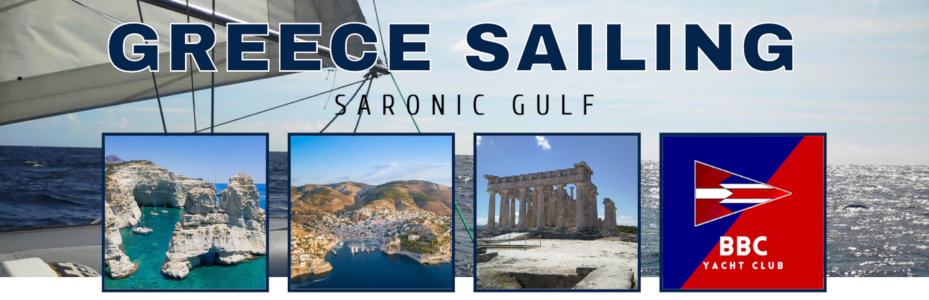
\includegraphics[scale=0.5]{../images/saronic_header_small.png} \\[0.2cm]
{\Huge \textsc{Notice to Mariners: \today}}\\
\line(1,0){450}
\end{center}


\begin{multicols}{2}

\noindent 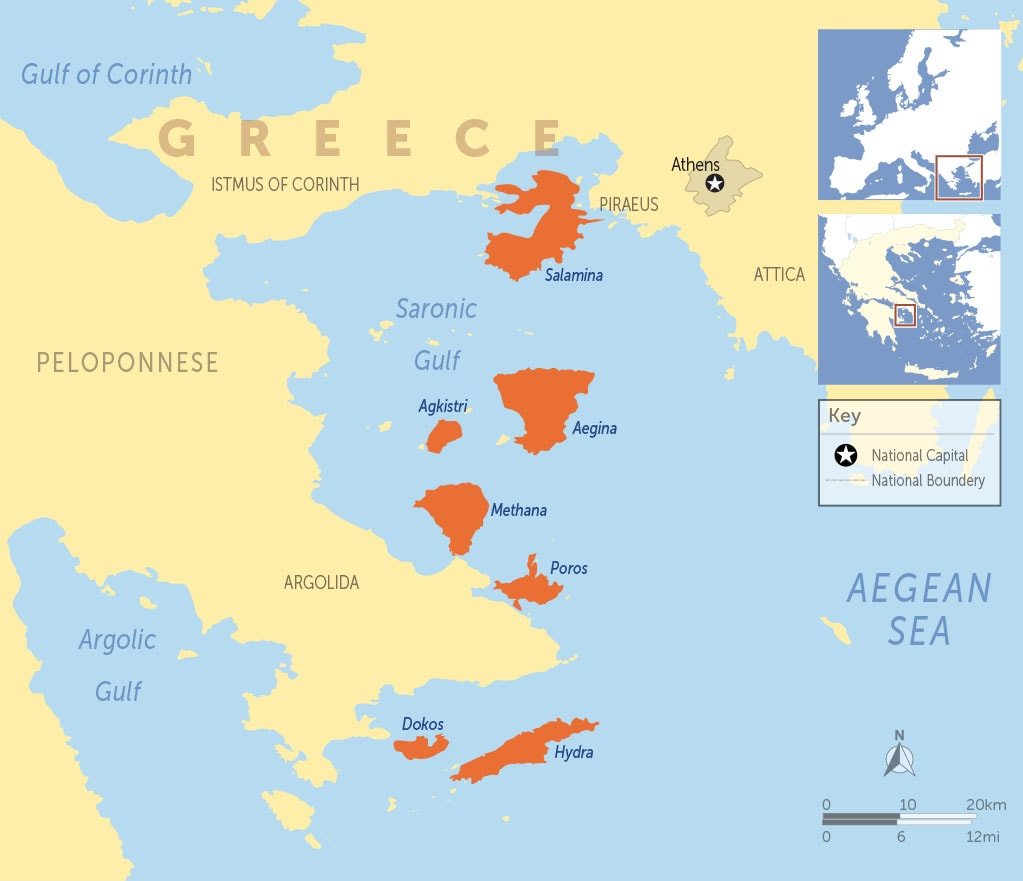
\includegraphics[scale=0.25]{saronic-map.jpg} 

\noindent Alimos ($ A\lambda\iota\mu o \sigma $) Marina is in the SW of Athens near Piraeus ($ \Pi\epsilon\iota\rho\alpha\iota\alpha\sigma $) Port on the Attica peninsular.\\
The sailing area consists of the Saronic and Argolic Gulfs (between the Attica and Peloponese peninsulars on the mainland) and islands such as Aegina, Poros, Methana, Hydra and Dhokos.  It includes small fishing villages, flooded volcanoes, artist retreats and some ancient sites.  Expect lots of time to look around, go snorkelling or diving, some culinary treats and not many marinas.


\section*{Travel}
\subsection*{Nearest Airport}
Athens International Airport Eleftherios Venizelos

\subsection*{Getting to the Marina}
\subsubsection*{Option 1}
Get a Taxi from the airport.  Arrivals Exit 3.  All official taxis are yellow, have a rooftop Taxi sign.  Tarrifs depend on your arrival time at the destination, not the time you departed.
\subsubsection*{Option 2}
Take Metro M3 to Syntagma ($\Sigma\upsilon\nu\tau\alpha\gamma\mu\alpha$) and then Tram 6 to Marina Alimou ($M\alpha\rho\iota\nu\alpha A\lambda\iota\mu\omicron\upsilon $) or Pikrodaphne ($P\iota\kappa\rho o \delta\alpha\phi\nu\epsilon $).
\subsubsection*{Option 3}
Take bus X96 to 1e Kalamikoy ($1\epsilon$ $K\alpha\lambda\alpha\mu\alpha\kappa\iota o \upsilon$).

\subsection*{Meeting Point}

\noindent Dia Noche (café in the marina complex near the swimming pool) at 16:00 on Saturday 30th.

\noindent At 17:00 skippers and 1 crew member have a meeting with Kiriacoulis representatives to complete check out paperwork and inventories.  Other crew will need to go to the supermarket.

\subsection*{Supermarkets near Marina}
NB Supermarkets are closed on Sundays!
\begin{itemize}
\item Galaxias, Leof. Eleftherias 35
\item Spar Express, R. Feraiou 2
\item Market In, Leof. Eleftherias 14
\item Sklavenitis, Thoukididou 42
\end{itemize}


\subsection*{Travelling with Lifejackets}
From the Civil Aviation Authority:\\

Small cartridges fitted into a self-inflating life-jacket must be for inflation purposes.

No more than two small cylinders of carbon dioxide or another suitable non-flammable non-toxic gas fitted in the life-jacket per person and a maximum of two spare cartridges.

\begin{itemize}
\item Carry on baggage - Yes
\item Checked baggage - Yes
\item On one's person - Yes
\item Airline approval required - Yes
\end{itemize}

\subsection*{EU Entry Requirements}
You can be asked to show the following at immigration:
\begin{itemize}
\item Passport less than 9 years 6 months old with 6 months remaining and enough space for 2 stamps (1/2 page).
\item Travel insurance including repatriation cover (EHIC/GHIC can reduce the costs of cover required).  Please ensure it covers coastal yachting. 
\item Proof of sufficient funds - (\euro{}50 per person per day).
\item Return flight ticket.
\item Copy of prescription for any drugs being carried.
\end{itemize}


\end{multicols}

\begin{center}
\line(1,0){450}
\end{center}

\noindent Simon Thompson\\
BBCYC Greek Naviguesser

\end{document}